\section{Introduction}
\label{sec:intro} 
We rely more and more on large scale distributed systems every day. Examples of such systems include the Internet, scientific computation clusters, weather forecasting systems and cellular networks. The energy efficiency of most of these systems is obscenely bad~\cite{Jeyarani:2012:DIA:2148243.2148374,AlDaoud2012745,5621969}. For instance, the servers which are present at the core of such systems consume as much as 60\% of their peak power consumption when operating under no-load~\cite{10.1109/MC.2007.443}. Challenges of global warming as well as rising electricity prices have placed significant emphasis upon research to improve the energy efficiency of large scale distributed systems. In this paper, we focus on cellular networks, but the techniques formulated apply to many other systems as well.

Cellular networks consume several tens of TWhs of electrical energy
every year worldwide~\cite{Oh:Comm:2011}. The major sink of power in a cellular network are Base
Transceiver Stations (BTSs), accounting for 50\% to 90\% of
the total power
consumption~\cite{Louhi:2007:BTSPower:INTELEC,Oh:Comm:2011}. Our focus, therefore, in the present work is on reducing the electricity consumption in the BTSs.

Global System for Mobile Communication (GSM) cellular networks are quite widely deployed, especially in the developing world. In the present work, we focused on GSM cellular networks alone, but most of the results and techniques should be applicable with few changes to other cellular communication technologies as well. In a GSM network, every BTS is equipped with several transceivers (TRXs), each of
which is allocated a single frequency band for transmission and
reception of radio signals. Each TRX further uses time
multiplexing to handle up to 8 full-rate voice calls over its
assigned frequency band in GSM systems. A typical configuration
is ``6+6+6'' depicting a BTS serving three \textit{sectors}
each with six TRXs. Thus, a BTS offers a \textit{fixed} capacity, as
determined by the total number of TRXs installed. Sites are
deployed such that this fixed BTS capacity can handle the peak
traffic load. However, traffic peaks only for a short duration
dropping off to a much lower trough each day, which means that
the GSM networks are over-provisioned during
low-traffic regimes.

Over-provisioned BTSs would be fine if they were also
load-proportional, i.e., consumed little power at no traffic
load. However, according to~\cite{Peng:2011:BTSSaving:Mobicom}
the no-load power consumption can be as high as 95\% of that at
full load. With fixed BTS capacity that is over-provisioned for
low traffic loads, today's cellular networks are highly energy inefficient.

There are generally two approaches to increase cellular network
energy efficiency. First, a clean-slate redesign which includes
innovations in communication systems, circuits and components.
This approach is not attractive for existing GSM operators,
which are the most prevalent in the developing world and are
expected to stay as such for several years to come, primarily due to the required expensive upgrades. 
A second approach is to make optimizations to the existing system
and equipment to get an improvement in overall energy
efficiency. Our present work is aligned with this latter
philosophy.

One can improve the energy efficiency of a cellular network by
adapting its ``online'' capacity to changes in traffic load.
Recent work has proposed turning off base stations to reduce
energy consumption during times of low traffic
load~\cite{Louhi:2007:BTSPower:INTELEC,Oh:Comm:2011,Peng:2011:BTSSaving:Mobicom,He:CellularPower:JN:2012}.
However, our conversations with multiple network operators
indicate that they are reluctant to employ such techniques
citing three reasons:
\begin{itemize}
\item Power cycling of entire base stations is expected to
    reduce equipment life time.
\item Turning off some BTSs may require an increased uplink
    power which may not be handled by many low-cost/power-limited mobile
    stations (MSs). This raises a risk of customer churn and is
    not acceptable to the operators in cut-throat
    competition prevalent in today's market.
\item These techniques of turning off BTSs may
    underestimate the increase in power needed for indoor
    MSs.
\end{itemize}

Our conversations with
wireless providers reveal that during low traffic periods, they often use a feature available in most vendor's equipment that power-gates TRX circuits at locations that
serve very few customers. Huawei calls this feature \textit{TRX shutdown} while Ericsson calls it \textit{BTS power saving}. We use the latter term generically in this paper. Since BTS power consumption has a traffic-independent
component~\cite{Peng:2011:BTSSaving:Mobicom} that depends,
among other factors, on the number of active TRXs, deactivating
TRXs reduces the BTS power consumption. For instance, turning
off one TRX cuts down BTS power consumption anywhere from $20W$
to $100W$, depending upon the frequency band (900 or 1800) and
deployed
equipment~\cite{Lorincz:BTS-Measure:Sensors:2012,flexibsc}.
Thus, scaling a ``6+6+6'' to a ``2+2+2'' configuration, by deactivating 12
TRXs will result in a saving of
240W to 1200W on a single site. The decision to use \textit{BTS
power saving} feature is generally local to the BTS without any
coordinated effort at the network level.

\begin{figure}
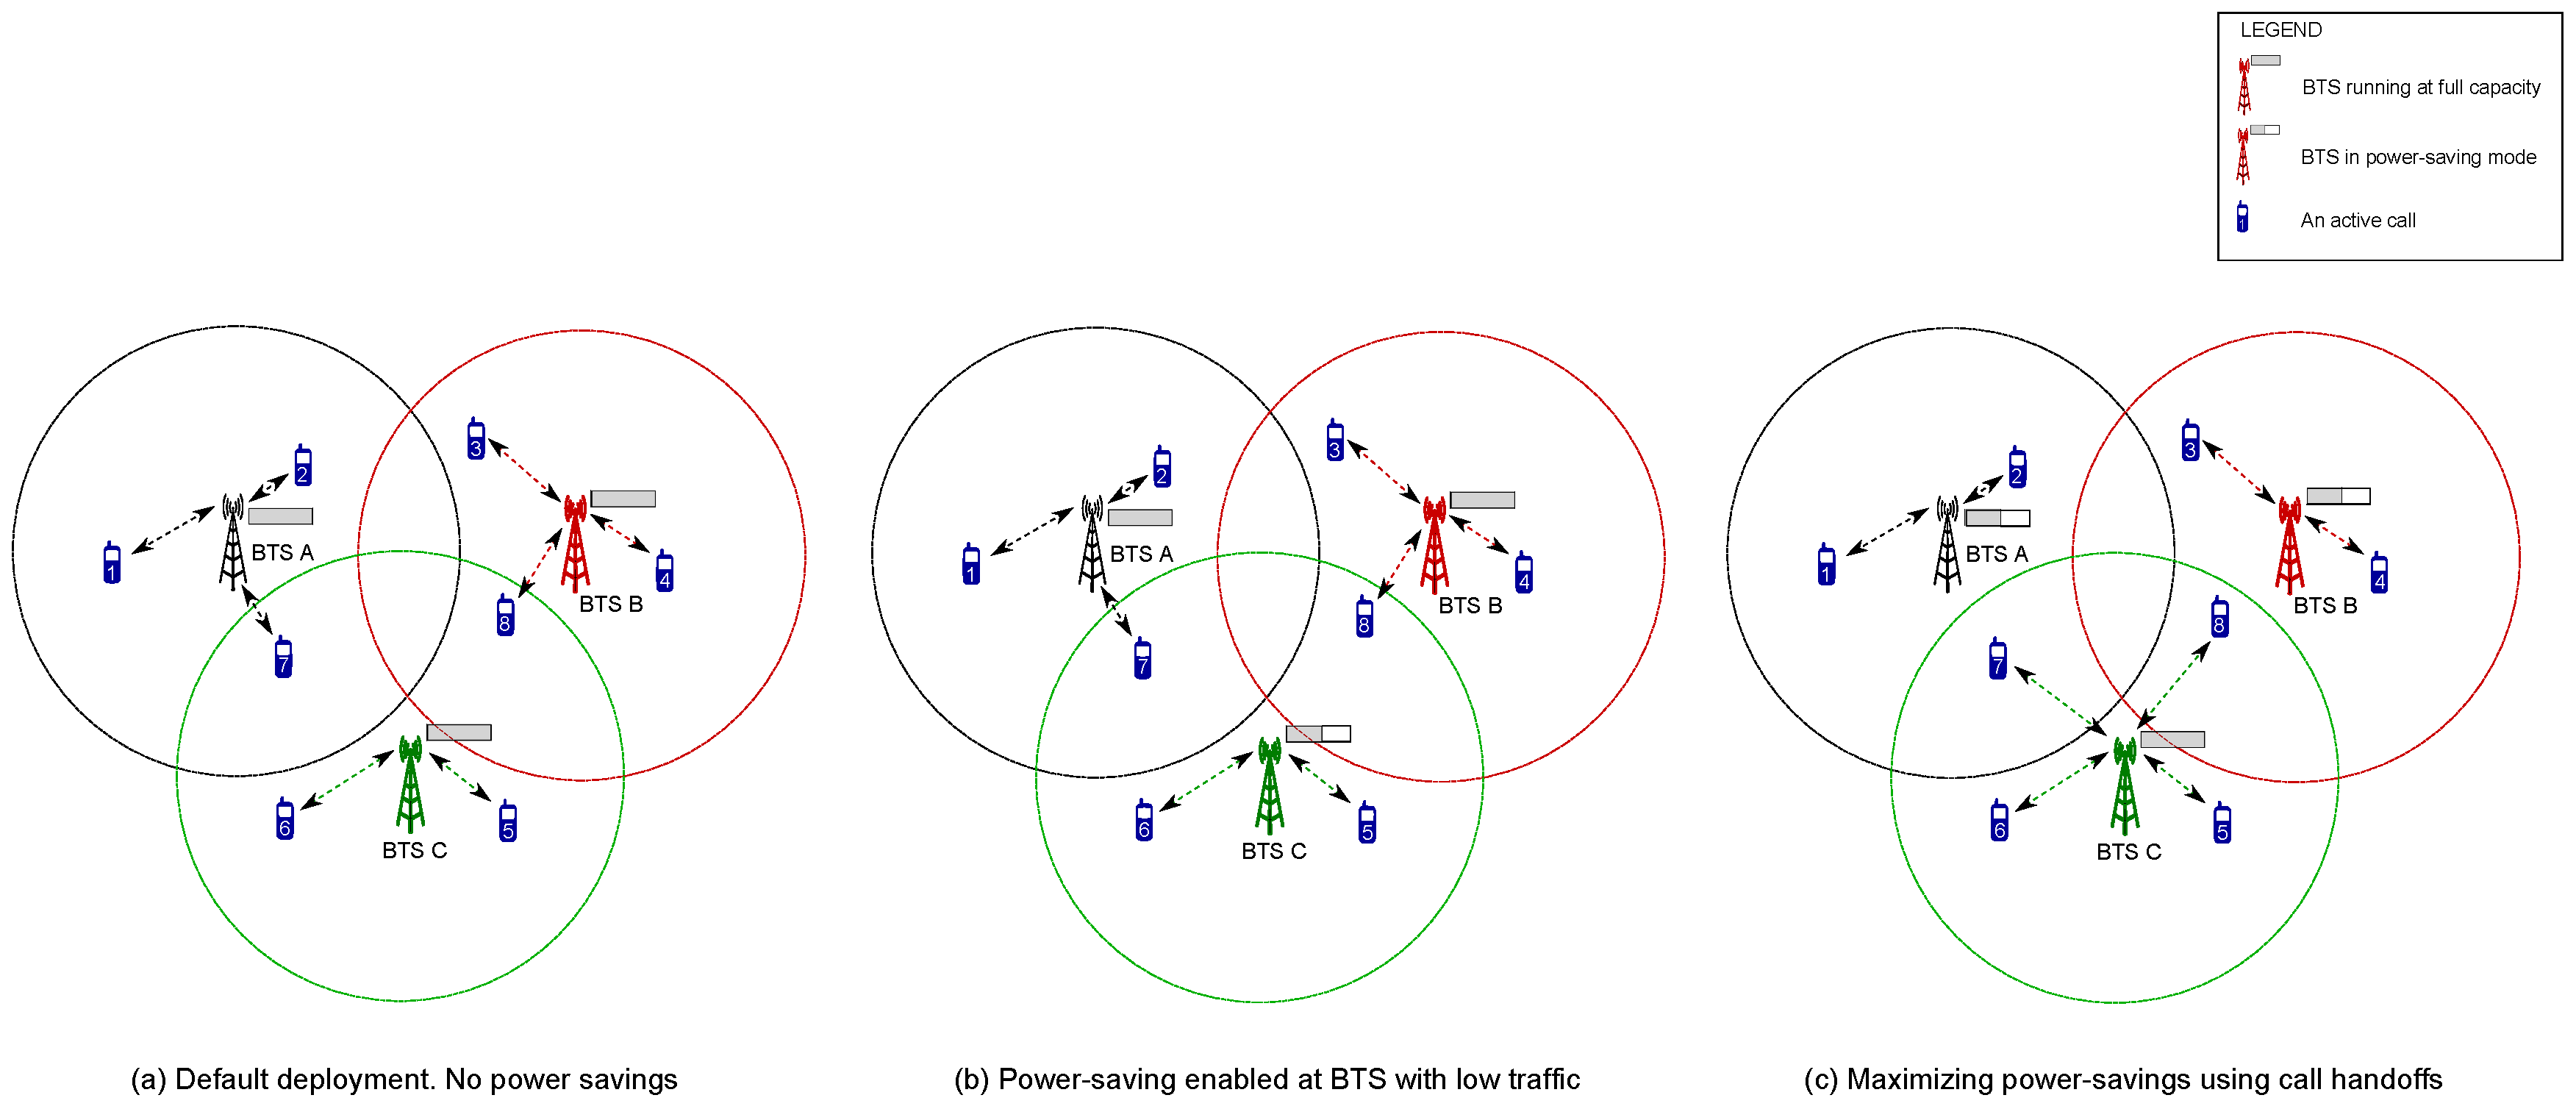
\includegraphics[width=1\textwidth]{figures/illustrationall.eps}
\caption{A toy example to illustrate the main idea behind Low-Carb. Three BTSs (A, B and C) are shown alongwith eight active calls. The serving BTS for each call is shown using a dashed line. A solid completely filled bar alongside a BTS symbol indicates that it is running in the default configuration where all TRXs are enabled. A BTS in power-saving mode is indicated with a half-filled bar next to it. Assume that power-saving mode may be enabled at a BTS if it has less than three active calls. (a) shows the default configuration where power-saving mode is not used. (b) shows the approach currently used by operators whereby power-saving mode is enabled on a BTS with low-traffic. (c) shows our proposed approach, whereby calls may be handed-off to nearby BTSs, thus maximizing the number of BTSs in power-saving mode.}
\label{fig:illustrationall}
\end{figure}


Let us illustrate the main idea behind the energy-saving approach proposed in this paper with the help of the illustration in Figure~\ref{fig:illusgtrationall}. The figure shows three nearby BTSs collectively serving eight active calls. The association of call to the serving BTS is indicated by means of a dashed line, while the boundary of the potential service area of a BTS is indicated by means of a dashed circle around it. Be default, each call is served by the BTS from which the mobile station receives the strongest signal. In this example, we assume that the call handling capacity of each BTS is six simultaneous calls. Furthermore, we assume that the power-saving threshold is three calls, i.e., if a BTS is serving less than three calls, it may be put into power-saving mode. In Figure~\ref{fig:illustrationall}, a BTS in it's default configuration, i.e., all TRXs enabled is indicated with a solid bar next to the BTS symbol. Meanwhile, a BTS in power-saving mode is shown by a half-filled bar next to the BTS symbol.


In Figure~\ref{fig:illustrationall} note that calls 1 through 6 may only be served through one BTS, while call 7 may be served either by BTS A or C and call 8 may be served either by BTS B or C. Figure~\ref{fig:illustrationall} (a) shows the default deployment where the default call routing and no power-saving is used. Since BTS C is serving only two calls, it may be placed in power-saving mode. Figure~\ref{fig:illustrationall} (b) shows this state, which indicates the current practice in operational cellular networks, whereby BTS C is put into power-saving mode because it's current call volume is below the power-saving threshold. However, this is not the optimal call routing strategy in terms of energy-savings. We may handoff calls 7 and 8 to BTS C, thereby reducing the call volume at both BTS A and B below the power-saving threshold. This results in the energy-optimal call routing strategy, proposed in this paper, shown in Figure~\ref{fig:illustrationall} (c). 


This paper presents Low-Carb which combines the \textit{BTS
power saving} with \textit{hand-off}, another commonly used
feature in cellular networks that facilitates user movement
from one location to another. Low-Carb proposes to hand-off
calls from one BTS to another, without making a negative impact
on the network quality of service, such that the \textit{BTS
power savings} can be applied to a maximal number of base
stations throughout the cellular network. As compared to the
use of uncoordinated \textit{BTS power savings}, Low-Carb
offers additional power savings as it may allow a larger number
of TRXs to be deactivated. 
In present day deployments, this is possible since most callers
receive sufficiently strong signal from several nearby
BTSs~\cite{Peng:2011:BTSSaving:Mobicom}. Fig.~\ref{fig:btscdf}
shows coverage diversity evident in the urban data from a large
cellular provider that we used in our evaluations; one can see
that about half of the callers have 3 or more candidates for
serving BTS. This fact alone, however, would not result in additional energy savings. Fortunately, neighboring sites can have different traffic loads at a given time. Fig.~\ref{fig:traffic}, for instance, shows normalized traffic at two neighboring sites in our dataset for a 24 hour period.

\begin{figure}
\centering
\subfigure[]{
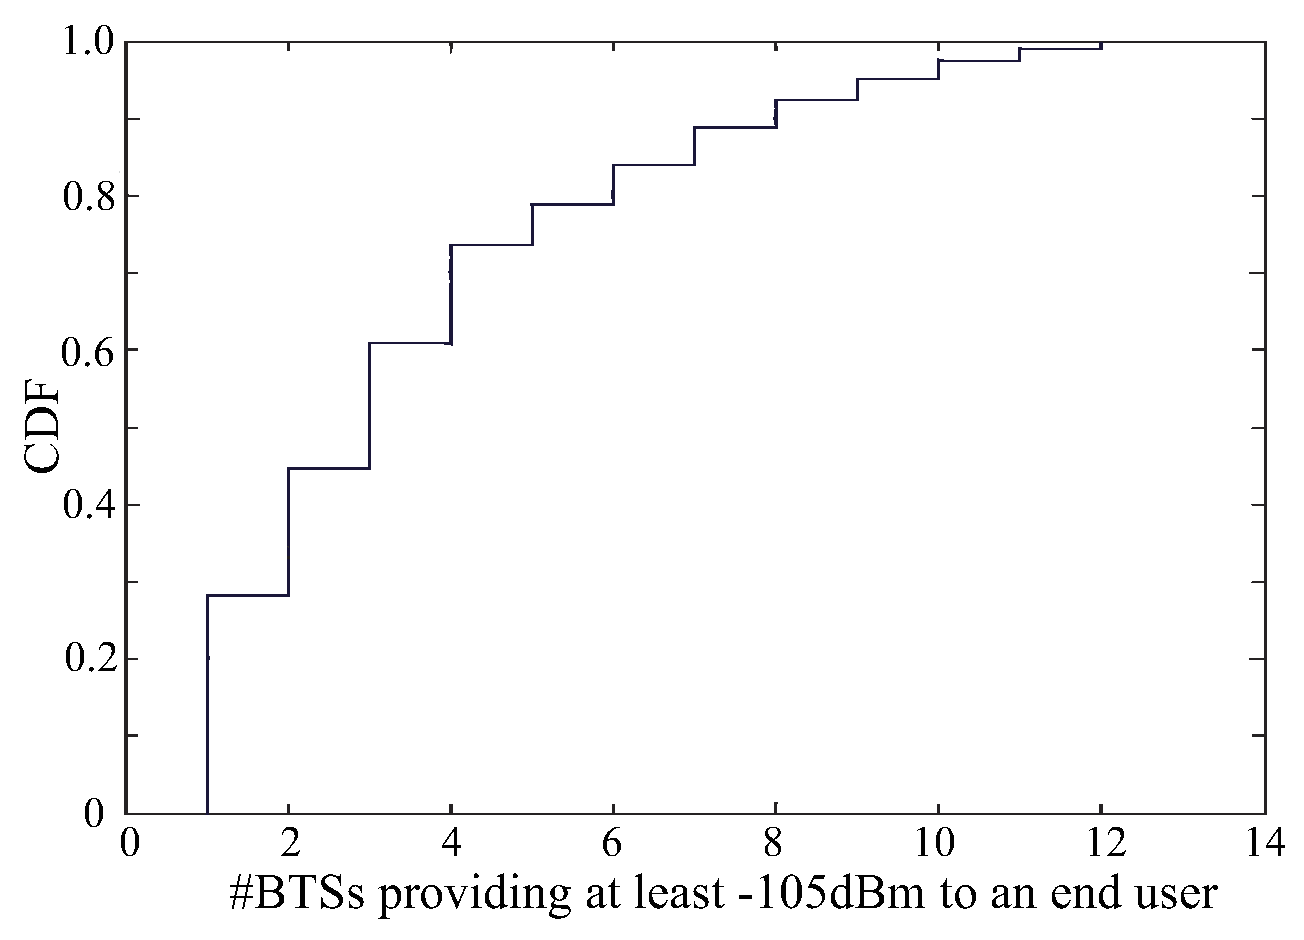
\includegraphics[width=0.48\textwidth]{figures/coveragecdf.eps}
\label{fig:btscdf}
}
\subfigure[]{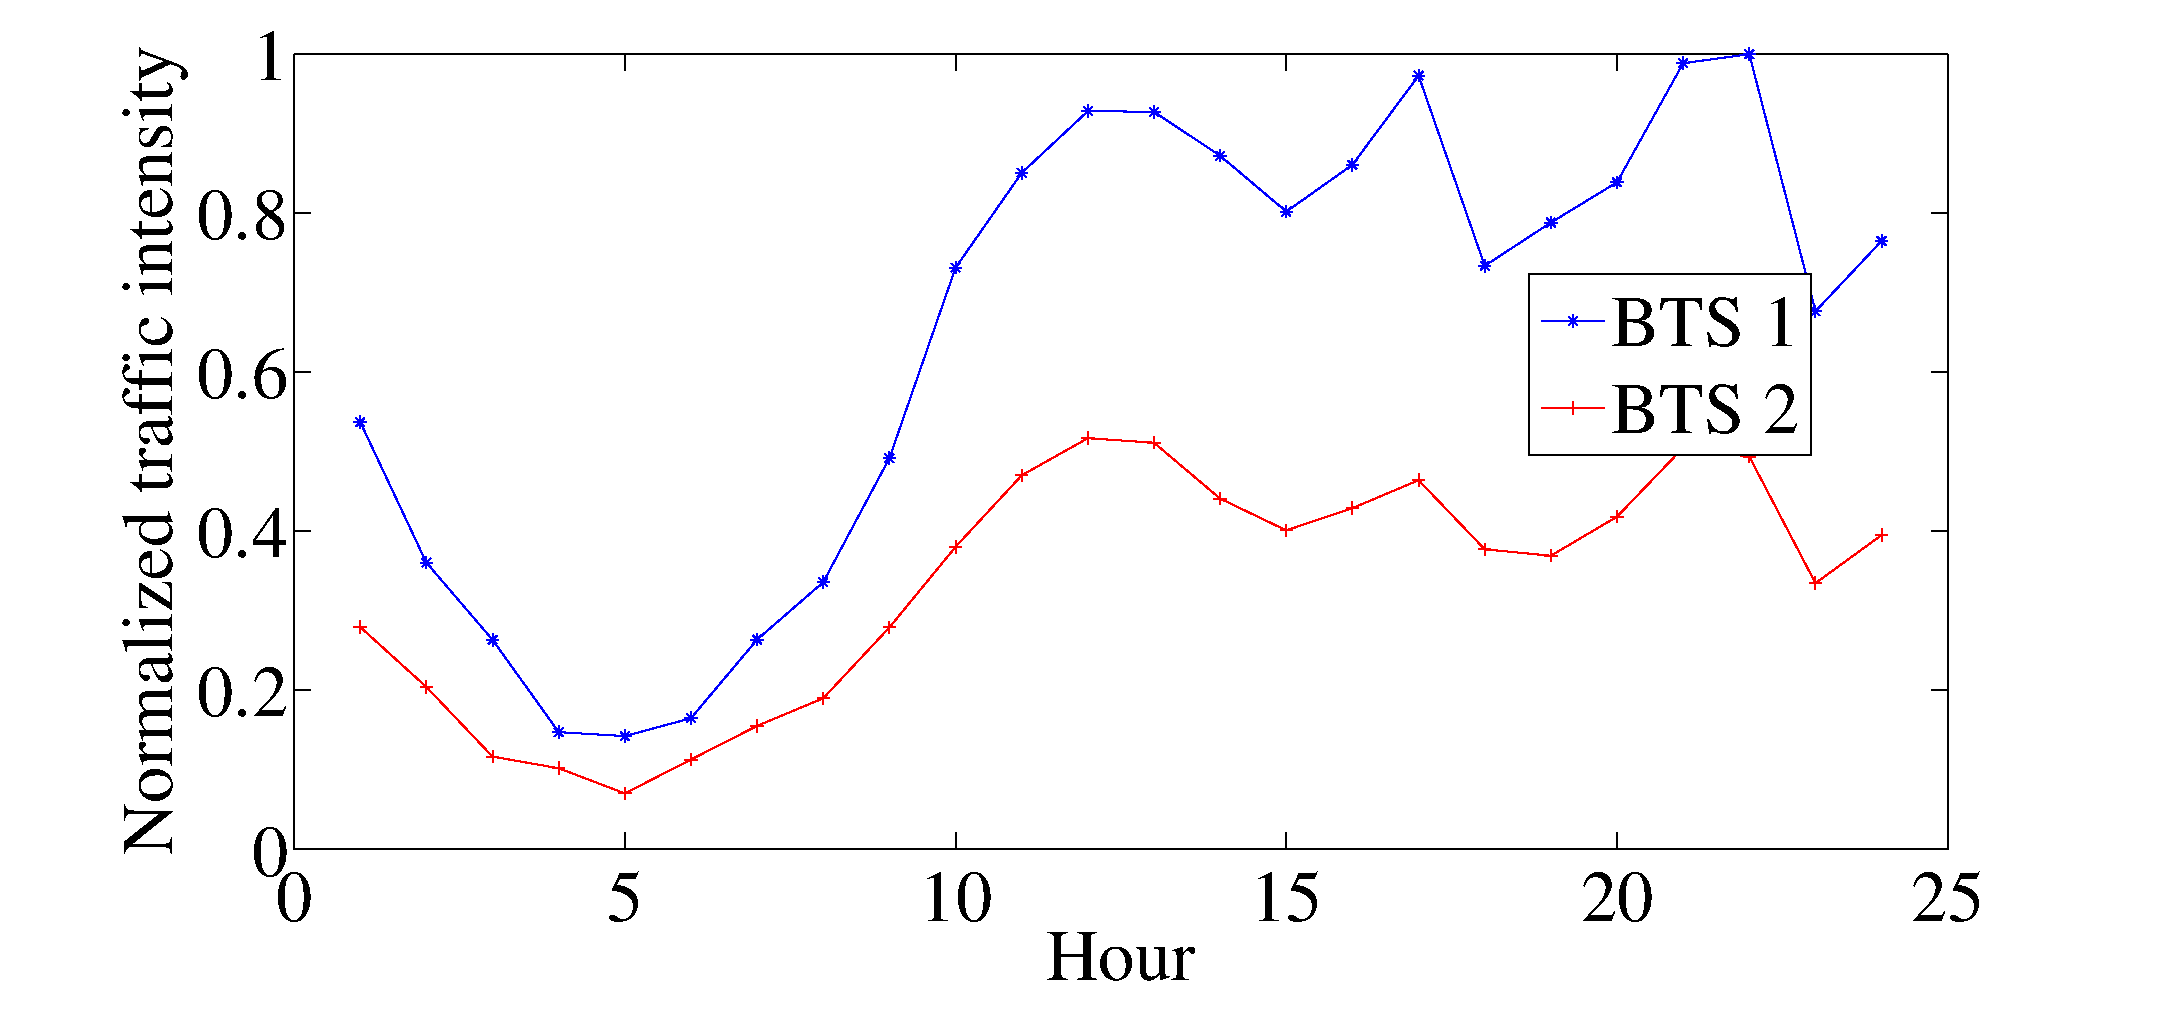
\includegraphics[width=0.48\textwidth]{figures/traffic.eps}
\label{fig:traffic}
}
\caption{Characteristics of our dataset: (a) Empirical CDF of the number of potential serving BTSs for a call in our dataset (large metropolitan area), (b) Normalized traffic intensity at two neighboring sites in our dataset} 
\label{fig:trafficmodelstats}
\end{figure}

We formulate an optimization problem to minimize the power
consumption in a GSM network by shuffling active calls between
nearby BTSs while keeping in check the MS uplink budget. Our
work is very similar in spirit to the concept of
\textit{frequency dimming}
in~\cite{Tipper:Dimming:Globecom:2010} albeit at a different
level of abstraction. A similar approach is also proposed
in~\cite{Blume:2010:BLTJ:CellularPower} with some rough
estimates of expected savings. We, on the other hand, use site
locations and traffic traces from a large cellular network with
more than 13 million subscribers to run a simulation study
assessing the benefits of dynamic equipment scaling coupled
with call hand-offs. A key benefit of our approach is that it 
does not require any additional hardware
and works within the GSM specifications.

The rest of the paper is structured as follows. The formulation
of Low-Carb optimization problem is given in
section~\ref{sec:formulation}. Experimental setup and the
results are presented in sections~\ref{sec:expermintalsetup}
and~\ref{sec:results}, respectively. In
section~\ref{sec:conclusions}, we draw the conclusions
highlighting the power saving strategy for providers.